%&latex
\documentclass{article}
\usepackage[utf8]{inputenc}
\usepackage[T1]{fontenc}
\usepackage[portuguese]{babel}
\usepackage{graphicx}
\usepackage{amsmath}
\usepackage{amssymb}

%% ---------------------------------------------------------------------------------------------------LISTAGEM
\usepackage{color}
\usepackage{listings}
\usepackage{courier}
\lstset{ basicstyle=\scriptsize\ttfamily, % Standardschrift
         numbers=left,                    % Ort der Zeilennummern
         numberstyle=\tiny,               % Stil der Zeilennummern
         stepnumber=1,                    % Abstand zwischen den Zeilennummern
         numbersep=5pt,                   % Abstand der Nummern zum Text
         tabsize=2,                       % Groesse von Tabs
         extendedchars=true,              %
         breaklines=true,                 % Zeilen werden Umgebrochen
         keywordstyle=\bfseries,         
         stringstyle=\ttfamily,           % Farbe der String
         showspaces=false,                % Leerzeichen anzeigen ?
         showtabs=false,                  % Tabs anzeigen ?
         xleftmargin=17pt,
         framexleftmargin=17pt,
         framexrightmargin=5pt,
         framexbottommargin=4pt,
         %backgroundcolor=\color{lightgray},
         showstringspaces=false,          % Leerzeichen in Strings anzeigen?
         frame=lines                      %hnone|leftline|topline|bottomline|lines|single|shadowboxi
 }
%% ---------------------------------------------------------------------------------------------------LISTAGEM

\lstdefinelanguage{Arduino}
{
morekeywords={volatile,include,LED_BUILTIN,INPUT_PULLUP,FALLING,sleep_enable,set_sleep_mode,sleep_disable,sleep_cpu,SLEEP_MODE_PWR_DOWN,cli,CS12,TOIE1,TCCR1A,TCCR1B,TCNT1,TIMSK1,digitalRead,false,true,if,attachInterrupt,detachInterrupt,digitalPinToInterrupt,CHANGE,sei,define,delayMicroseconds,analogRead,analogReference,available,DEFAULT,int,read,setup,loop,pinMode,digitalWrite,delay,HIGH,LOW,void,OUTPUT,Serial,
begin, println,print,for,byte,return},
sensitive=true,
morecomment=[l]{//,/*,*/},
morestring=[b]",
}

\usepackage{hyperref}

\begin{document}

%+Title
\title{Sistema de Medida de Forças com Células de Carga e ESP32}
\author{João Paulo Coelho}
\date{\today}
\maketitle
%-Title

%+Abstract
\begin{abstract}
    Logbook para referência. 
\end{abstract}
%-Abstract

%+Contents
\tableofcontents
%-Contents

\section{Introdução}

Algumas questões que é preciso responder:
\begin{itemize}
\item 
Quantas células de carga são necessárias?
\item
Qual a frequência de amostragem?
\item
Durante quanto tempo os ensaios são realizados?
\item 
Descrição do processo?
\item

\end{itemize}
\section{Instalação do ESP32}
\begin{enumerate}
\item 
Abrir a janela de preferências do Arduino IDE. Para isso, navegar através do menu ``Ficheiro'' até ao item ``Preferências''.

%--------------------------------------------------------------------------------
\begin{figure}[htb!]
\centering
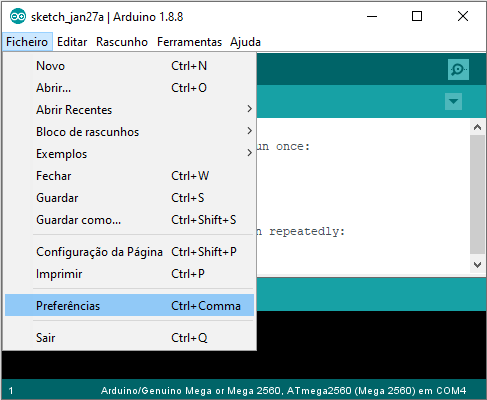
\includegraphics[width=0.5\textwidth]{Figuras/Fig1.png}
\label{fig:fig1}
\end{figure}
%--------------------------------------------------------------------------------
\item
Escrever no campo ``URL Adicionais do Gestor de Placas o seguinte endereço:
\begin{verbatim}
https://dl.espressif.com/dl/package_esp32_index.json
\end{verbatim}
%--------------------------------------------------------------------------------
\begin{figure}[htb!]
\centering
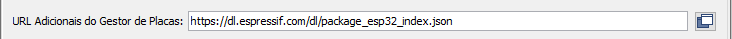
\includegraphics[width=1\textwidth]{Figuras/Fig2.png}
\label{fig:fig2}
\end{figure}
%--------------------------------------------------------------------------------
\item
Abrir o gestor de placas em ``Ferramentas'' e selecionar ``Gestor de Placas''.
%--------------------------------------------------------------------------------
\begin{figure}[htb!]
\centering
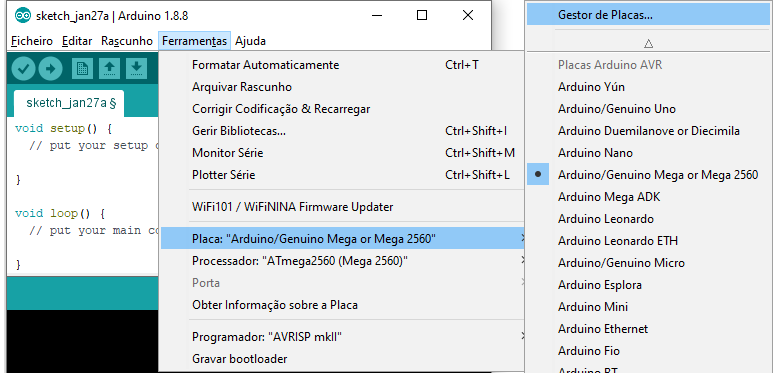
\includegraphics[width=0.7\textwidth]{Figuras/Fig3.png}
\label{fig:fig3}
\end{figure}
%--------------------------------------------------------------------------------

\item
Procurar por ESP32 e instalar ``ESP32 by Espressif Systems''
%--------------------------------------------------------------------------------
\begin{figure}[htb!]
\centering
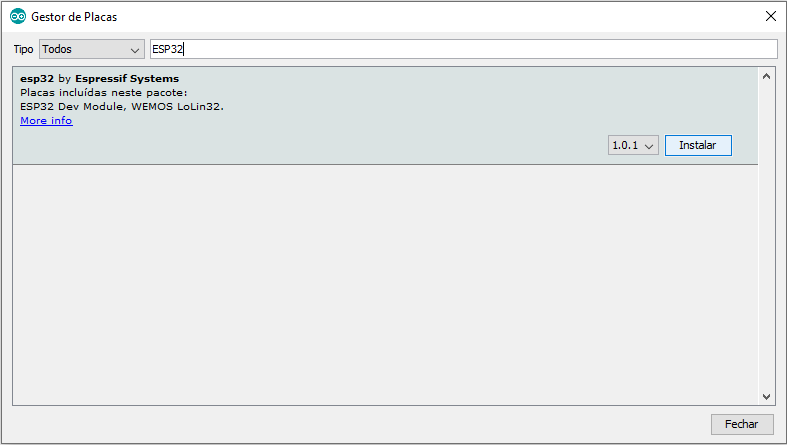
\includegraphics[width=0.7\textwidth]{Figuras/Fig4.png}
\label{fig:fig4}
\end{figure}
%--------------------------------------------------------------------------------
%--------------------------------------------------------------------------------
\begin{figure}[htb!]
\centering
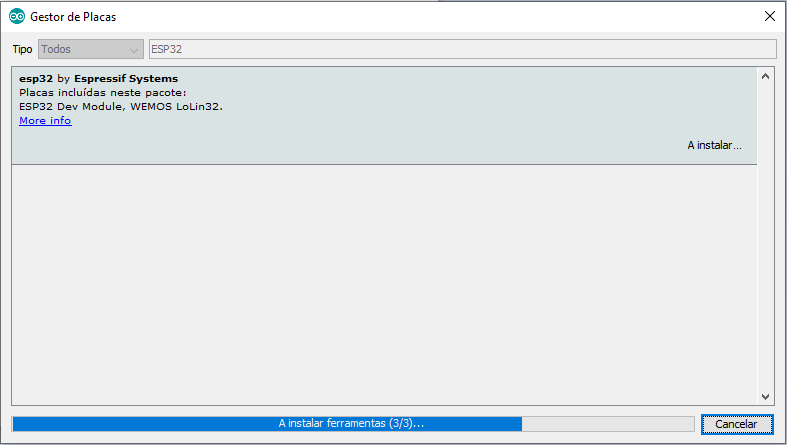
\includegraphics[width=0.7\textwidth]{Figuras/Fig5.png}
\label{fig:fig5}
\end{figure}
%--------------------------------------------------------------------------------
\end{enumerate}

\subsection{Teste da Instalação}
\begin{enumerate}
\item 
Ligar a placa de desenvolvimento ESP32 ao computador através de um cabo micro USB.
%--------------------------------------------------------------------------------
\begin{figure}[htb!]
\centering
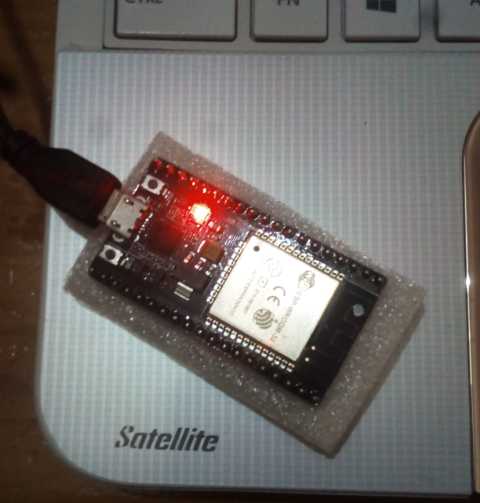
\includegraphics[width=0.45\textwidth]{Figuras/Fig7.png}
\label{fig:fig7}
\end{figure}
%--------------------------------------------------------------------------------
\item
No Arduino IDE selecionar a placa e o porto de comunicação.
%--------------------------------------------------------------------------------
\begin{figure}[htb!]
\centering
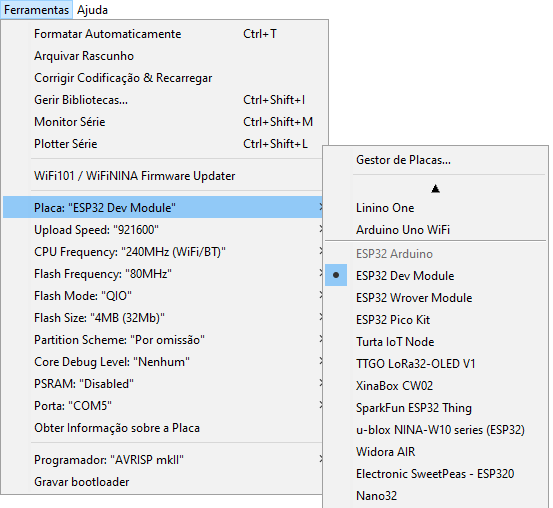
\includegraphics[width=0.7\textwidth]{Figuras/Fig6.png}
\label{fig:fig6}
\end{figure}
%--------------------------------------------------------------------------------
\item
Carregar o programa apresentado na listagem \ref{list1} para a plataforma de desenvolvimento e comprovar o seu funcionamento.
\lstinputlisting[float, language=Arduino,label=list1,caption=Exemplo de um programa elementar para testar a placa e a instalação do ESP32 no IDE do Arduino.]{Firmware/Teste1/Teste1.ino}

Outro teste que pode ser executado é aquele que aparece nos exemplos como WiFiScan. A listagem do programa é:
\lstinputlisting[float, language=Arduino,label=list1,caption=Exemplo de um programa elementar para testar a placa e a instalação do ESP32 no IDE do Arduino.]{Firmware/Teste2/Teste2.ino}
e o resultado da sua execução, para este caso particular, é:
%--------------------------------------------------------------------------------
\begin{figure}[htb!]
\centering
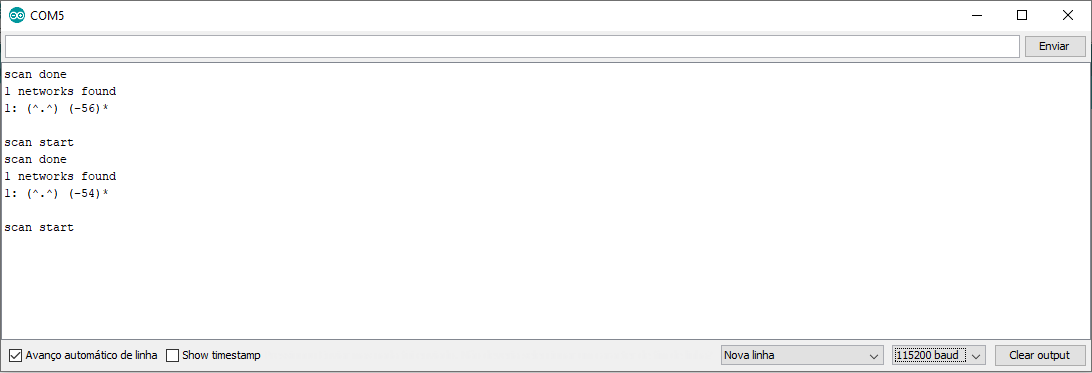
\includegraphics[width=0.7\textwidth]{Figuras/Fig9.png}
\label{fig:fig6}
\end{figure}
%--------------------------------------------------------------------------------

\end{enumerate}

\section{Célula de Carga}

A célula de carga utilizada nestes ensaios é um transdutor com referência 3140 e uma capacidade de 500~kg tanto à tração como à compressão. Esta célula de carga foi adquirida no site \url{https://www.robotshop.com/eu/en/500kg-s-type-load-cell.html} por cerca de 60 euros. O aspeto dela, assim como as suas dimensões mecânicas, está representada na figura \ref{fig:fig11}.

%--------------------------------------------------------------------------------
\begin{figure}[htb!]
\centering
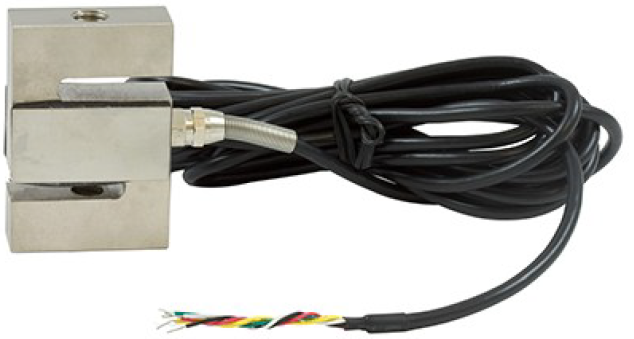
\includegraphics[width=0.45\textwidth]{Figuras/Fig11.png}
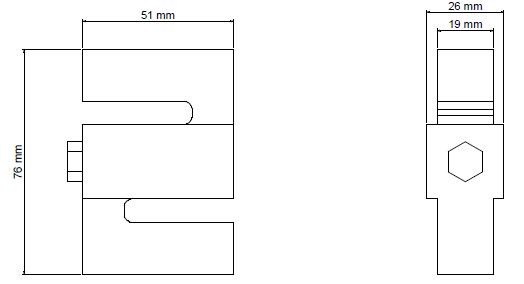
\includegraphics[width=0.45\textwidth]{Figuras/Fig14.png}
\label{fig:fig11}
\end{figure}
%--------------------------------------------------------------------------------

\subsection{Características Metrológicas}

As características metrológicas do sensor encontram-se sumariadas na tabela representada na Figura \ref{fig:fig10}.

%--------------------------------------------------------------------------------
\begin{figure}[htb!]
\centering
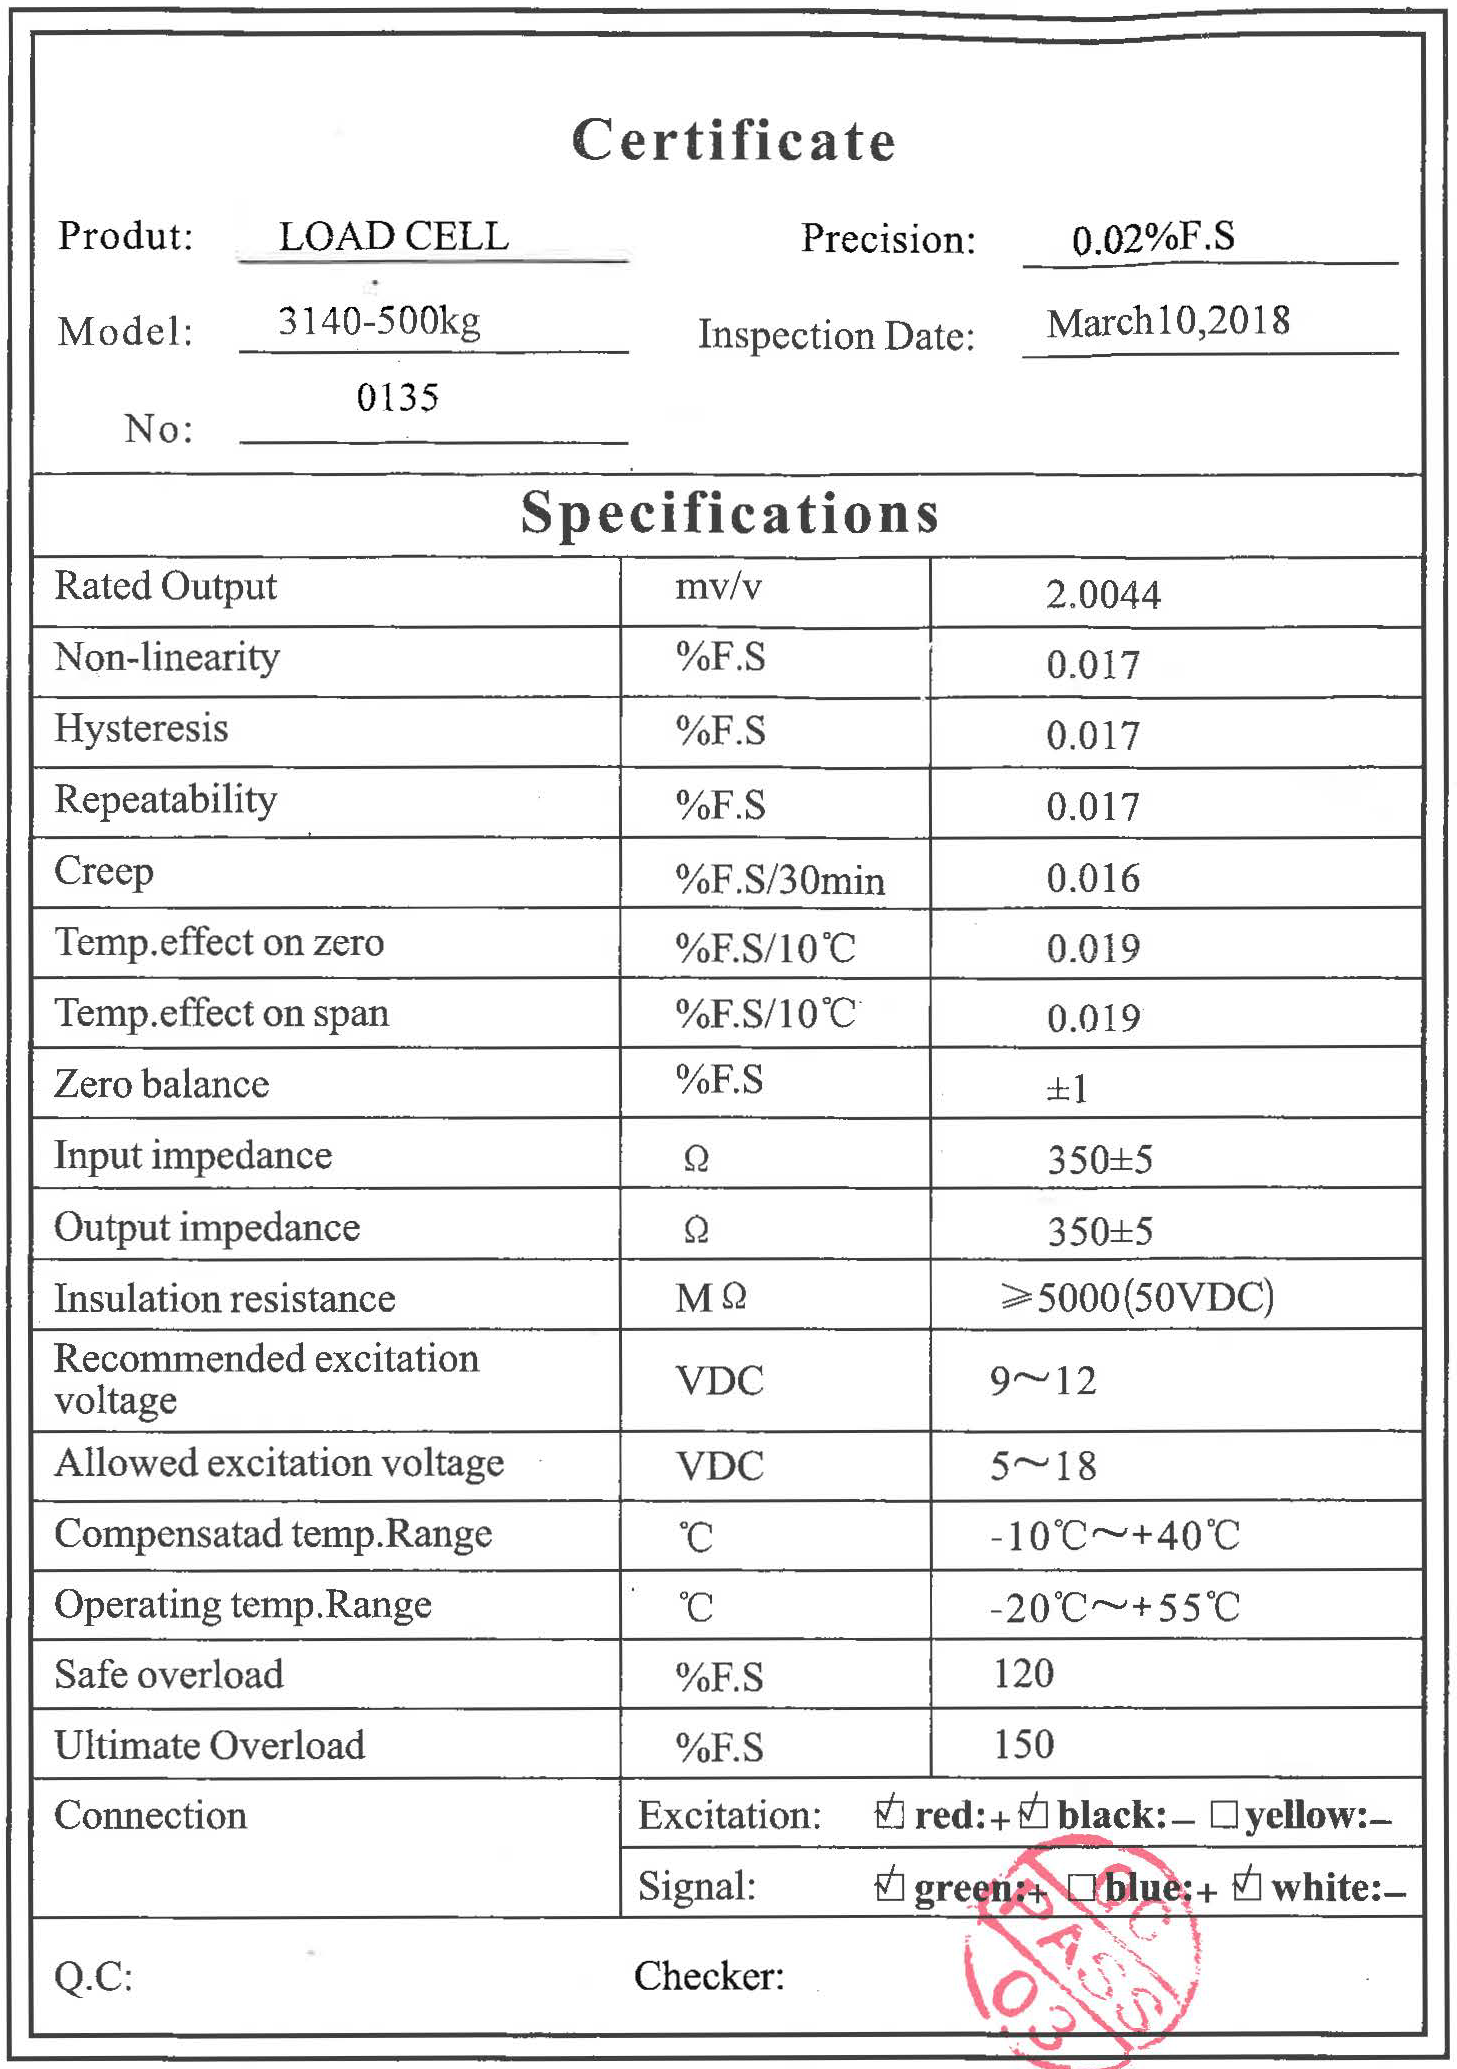
\includegraphics[width=0.65\textwidth]{Figuras/Fig10.png}
\label{fig:fig10}
\end{figure}
%--------------------------------------------------------------------------------

De acordo com as especificações apresentadas nessa tabela, observa-se que:
\begin{description}
\item[Overload:] O valor máximo se sobrecarga é de 120\% do valor de fim-de-escala (FdE) que neste caso é 500~kg. Por isso, esse valor é de 600~kg. O valor limite de sobrecarga é 150\% do valor de FdE ou seja 750~kg.

\item[Sensibilidade:] A sensibilidade $S$ desta célula de carga é de 2.0044~mV/V. Isto significa que, a cada Volt aplicado à tensão de alimentação, a tensão de desiquilíbrio da célula quando excitada pela carga máxima é igual a 2.0044~mV. Ou seja, se $V_o$ for a tensão de desiquilíbrio da ponte de extensómetros da célula de carga, e se $V_{CC}$ for a tensão de polarização dessa ponte então,
\begin{equation}
V_o = \frac{F}{FdE} \times S\times V_{CC}
\end{equation}

Assim, se a ponte for alimentada com 3.3~V, o valor de $V_o$, em mV, é dado por:

\begin{equation}
V_o\approx 0.01323\times F
\end{equation}

Ou seja, uma sensibilidade de 0.01323~mV por cada kg. Para o sistema de medida ter uma resolução de 1~kg é necessário que o conversor A/D tenha uma resolução superior a:
\begin{equation}
\frac{3.3}{2^n}\le\frac{0.01323}{1000}
\end{equation}

de onde se tira que:
\begin{equation}
n \ge \left\lceil\log_2\left( \frac{3.3\times 1000}{0.01323}\right)\right\rceil
\end{equation}
ou seja $n\ge 18$. Um conversor A/D de 24 bits terá a capacidade de distinguir variações no peso de:

\begin{equation}
\frac{3.3}{2^{24}}\approx 1.967\times 10^{-7}
\end{equation}
ou seja, uma resolução em torno de 0.2~mV. Esta tensão corresposponde à tensão de desiquilíbrio provocada por um peso de aproximadamente 15~kg.

Há que notar, entretanto, que o HX711 fornece um ganho programável entre 64 e 128. Considerando o ganho mais baixo, $V_o=0.8467\times F$ e logo o a resolução da balança será em torno das 250~g. Obviamente, para um ganho de 128 a resolução será perto de 125~g.

\item[Precisão:] O valor da precisão é descrita como sendo $\pm$ 0.02\% do valor de FdE. Como o valor de FdE é 500~kg, então a precisão é $\pm$0.1~kg ou seja $\pm$100~g.

\item[Repetibilidade:] A repetibilidade mede a capacidade do sistema fornecer informação consistente qunando excitado com o mesmo sinal. Neste caso, a repetibilidade é de 0.017\% do valor de fim-de-escala. Ou seja, cerca de 85 gramas. 

\item[Creep:] Diz respeito ao aumento no valor da saída ao fim de 30 minutos de aplicação de uma tração/compressão constante.


\end{description}

\subsection{Conectividade Elétrica}

A saída da célula de carga e disponibilizada em 5 fios de cores vermelho, verde, branco, preto e amarelo. As descrição de cada um desses fios está tabelada na Figura \ref{fig:fig12}. O condicionamento de sinal, nas folhas de dados da célula de carga, refere o dispositivo PhidgetBridge (\url{https://www.phidgets.com/?tier=3&catid=98&pcid=78&prodid=1027}). No entanto, neste protótipo iremos utilizar o HX711.

%--------------------------------------------------------------------------------
\begin{figure}[htb!]
\centering
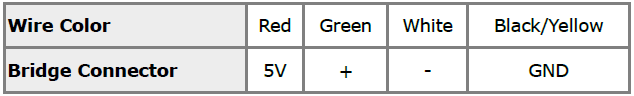
\includegraphics[width=0.65\textwidth]{Figuras/Fig12.png}
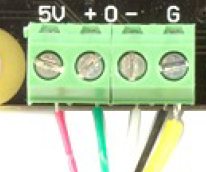
\includegraphics[width=0.2\textwidth]{Figuras/Fig13.png}
\label{fig:fig12}
\end{figure}
%--------------------------------------------------------------------------------


%--------------------------------------------------------------------------------
\begin{figure}[htb!]
\centering
\includegraphics[width=0.85\textwidth]{Figuras/Fig15.png}
\label{fig:fig15}
\end{figure}
%--------------------------------------------------------------------------------

\section{Arduino Pro Mini}
(\textbf{addon} - 28/03/2025)
 À data em que escrevo esta adição ao livro de campo, 6 anos depois deste projeto, tive que recondicionar os sistemas que entretanto foram construídos. Uma parte do trabalho está no EasyEda (esquema e PCB) e outra parte do trabalho em disco local. Criei agora um repositório no GIT para colocar algumas coisas.

O hardware construído assenta num Arduino Pro Mini pelo que a parte anterior relativa ao ESP32 acabou por não ser utilizada. A imagem da figura que se segue mostra o aspeto \textbf{final} de uma das 3 unidades que foram construídas.
%--------------------------------------------------------------------------------
\begin{figure}[htb!]
\centering
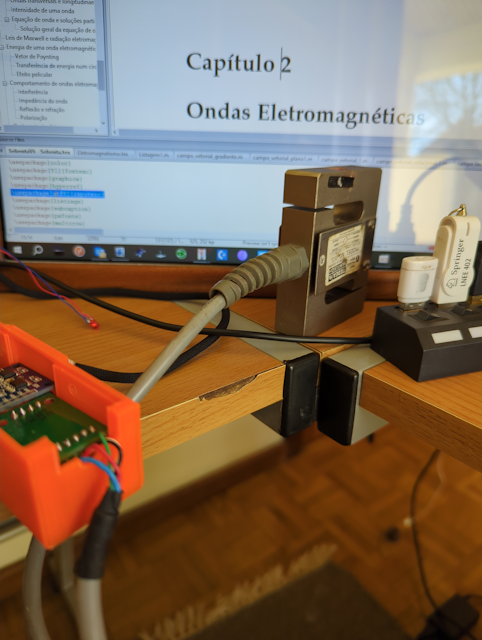
\includegraphics[width=0.4\textwidth]{Figuras/Fig28.png}
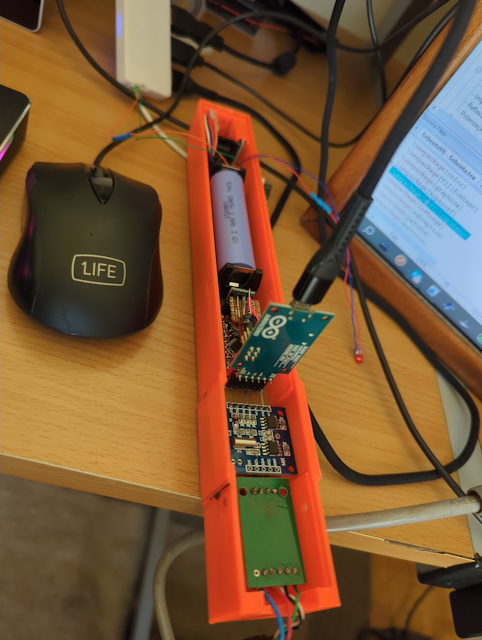
\includegraphics[width=0.4\textwidth]{Figuras/Fig29.png}
\label{fig:fig28}
\end{figure}
%--------------------------------------------------------------------------------

Como se pode ler na secção que se segue, o bootloader do Arduino foi alterado e, por isso, a plataforma não pode ser reprogramada com o Arduino IDE sem realizar os seguinte passos:
\begin{itemize}
\item 
Utilizar o Arduino IDE 1.6.0 - Para memória futura, uma versão desse software é mantido na paste
\item
Copiar o ficheiro ``boards.txt'', que se encontra no diretório ``Codigo'', para o diretório ``Progamas (x86)/Arduino/hardware/arduino''
%--------------------------------------------------------------------------------
\begin{figure}[htb!]
\centering
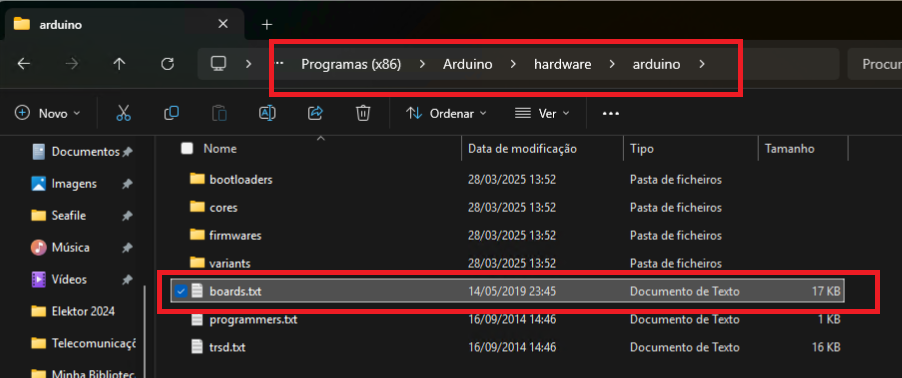
\includegraphics[width=0.7\textwidth]{Figuras/Fig31.png}
\label{fig:fig31}
\end{figure}
%--------------------------------------------------------------------------------
\item
Copiar Makefile e restantes dicheiros que se encontram no diretório ``Codigo'' para ``Programas (x86)/Arduino/hardware/bootloaders/optiboot''.
%--------------------------------------------------------------------------------
\begin{figure}[htb!]
\centering
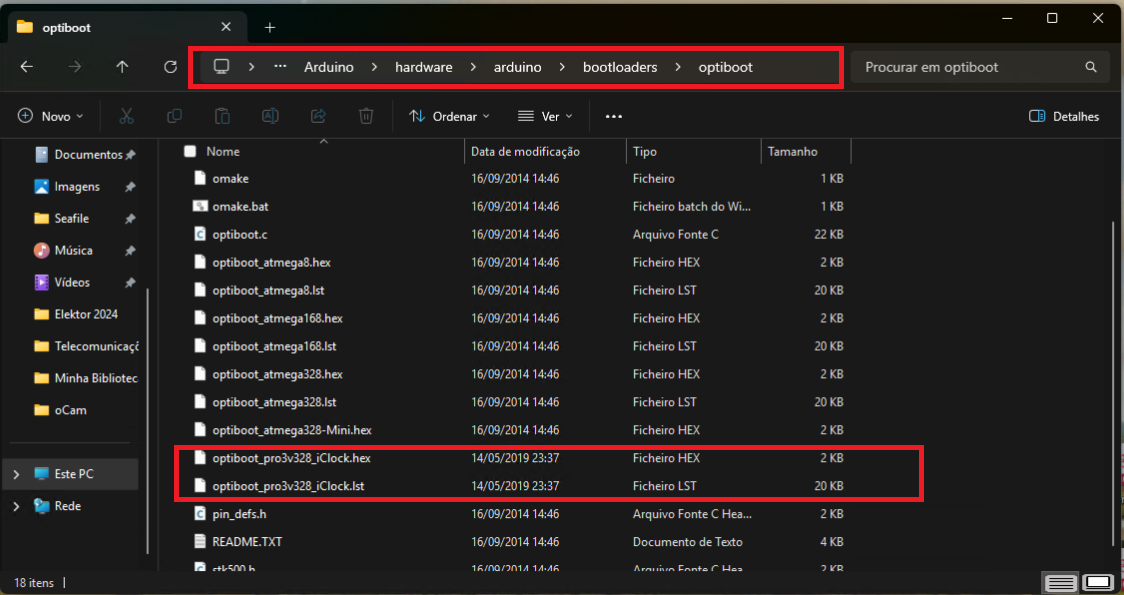
\includegraphics[width=0.8\textwidth]{Figuras/Fig30.png}
\label{fig:fig30}
\end{figure}
%--------------------------------------------------------------------------------
\end{itemize}
%
\subsection{Alterar para funcionar com clock interno}

Utilizar um arduino UNO como ISP:
\begin{itemize}
\item 
Connect the Uno to the PC (using USB)
\item
Open the Arduino IDE (I'm using v1.6.11)
\item
Check the board: Tools Menu -> Board ->Arduino Uno
\item
Check the port: Tools Menu -> Serial Port -> [select the port for the Uno]
\item
Load the ISP sketch: File menu -> Examples -> ArduinoISP ->ArduinoISP
\item
Upload - once complete, the Uno is configured as ISP
\item
Remove connection from Uno (power off)
\end{itemize}

Connect the two devices for programming:

\noindent Uno ------------------------Pro Mini\\
5V (vcc) ------------------- VCC\\
GND ------------------------GND\\
Pin 10 ---------------------- RST\\
Pin 11 ---------------------- Pin 11\\
Pin12 ---------------------- Pin 12\\
Pin 13 ------------------- -- Pin 13\\

Third step is to burn the bootloader:-


\begin{itemize}
\item 
Connect the Uno to the PC (Arduino IDE still open)
\item
Change the board: Tools Menu -> Board ->Arduino Pro or Pro Mini
\item
Check the speed and processor: Tools Menu -> Processor -> ATmega328 (5V, 16MHz)
\item
Choose the programmer> Tools Menu -> Programmer -> Arduino as ISP
\item
Burn the bootloader: Tools Menu -> Burn Bootloader
\end{itemize}

\subsubsection{Notas}

Para criar um novo bootloader é necessário ter o ``make'' instaldo que, a partir da versão do Arduino 1.0.6 não vem instaldo. Por isso, essa versão do Arduino foi instalada e o bootloader criado. Os ficheiros no diretório Codigo/Bootloader são os ficheiros produzidos no processo de criação do booloader. O ficheiro ``boards.txt'' deve substituir o homónimo na pasta criada durante a instalação do Arduino. O ficheiro ``Makefile'' assim como o ``.hex'' e o ``.lst'' serão colocados na pasta ``optiboot''.

De acordo com a informação fornecida pela Microchip, o ponto de operação definido pela frequência de clock e tensão de alimentação deve ser mantida dentro da região sobreada do gráfico da Figura.

%--------------------------------------------------------------------------------
\begin{figure}[htb!]
\centering
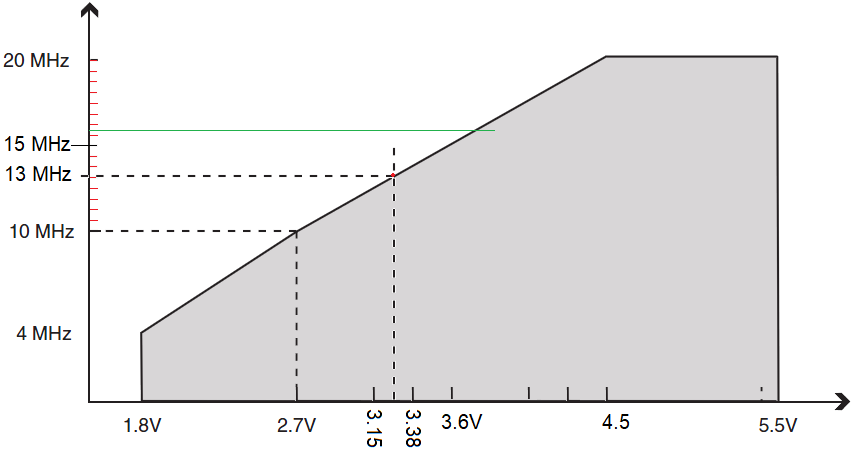
\includegraphics[width=0.85\textwidth]{Figuras/Fig16.png}
\label{fig:fig15}
\end{figure}
%--------------------------------------------------------------------------------

A frequência de 16 MHZ é demasiado elevada para uma utilização estável do microcontrolador. Como a placa que foi adquirida utiliza um cristal de 16 MHz, a única alternativa é recorrer ao oscilador interno. no entanto, por defeito não é possível definir o clock interno como fonte do sinal de sincronismo. Para isso, foi necessário criar um novo bootloader. Depois de se criar o Makefile e o boards.txt, bastou escrever, dentro da pasta optiboot, o comando:\\

\texttt{omake pro3v328\_iClock}.\\

Utilizando um arduino UNO como progamador ISP carregou-se o bootloader para o Arduino Pro Mini.
%--------------------------------------------------------------------------------
\begin{figure}[htb!]
\centering
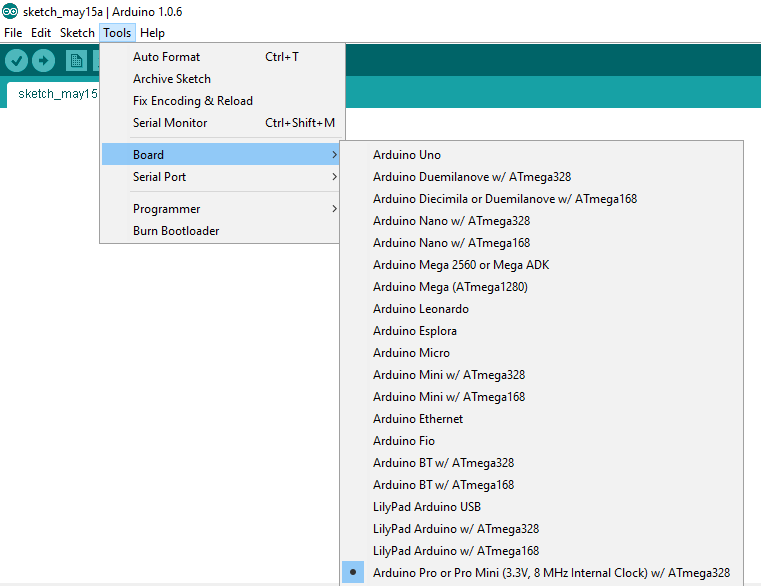
\includegraphics[width=0.85\textwidth]{Figuras/Fig20.png}
\label{fig:fig15}
\end{figure}
%--------------------------------------------------------------------------------

\subsection{Modo Sleep}

Uno uses between 30-40 mA when awake and about 19 mA when asleep. The Pro Mini uses 25mA when awake and 0.57 mA when asleep

\lstinputlisting[float, language=Arduino,label=list1,caption=Sleep well my sweet prince....]{Codigo/Sleep/Sleep.ino}

Este programa executa a seguinte operação: o Arduino arranca e ``acorda por 5 segundos''. Sempre que ele está acordado o LED integrado na placa encontra-se aceso. Ao fim desses 5 segundos, o CPU adormece e assim permanece até uma transição do nível alto para o nível baixo no pino 2 seja sentida. Quando isso acontece, o arduino sai do modo sleep, desabilita as interrupções e permanece acordado 5 segundos ao fim dos quais volta a adormecer.


Dos ensaios feitos, verificou-se que durante o modo SLEEP, a plataforma consumia um total de 5~mA quando alimentado por uma tensão de 5~V e uma frequência de clock de 8~MHz fornecida pelo oscilador interno. Penso que essa corrente elétrica se deve ao LED pelo que vamos ter que o dessoldar. No modo normal consome perto de 15.5~mA.        

Quando alimentado por uma tensão de 3.3~V, o valor da corrente consumida no modo normal desce para 6.5~mA. No modo sleep esse valor desce para 2.98~mA.

De acordo com alguns esquemas que vi na NET, a resistência de polarizção do LED\ vermelho é 10~k$\Omega$ e a resistência de polarização do LED verde igual a 330~$\Omega$.
 
Ora vamos fazer umas contas: Para uma tensão de 5~V, e considerando que o Arduino no modo SLEEP consome 0~mA, então:
\begin{equation}
\begin{split}
V &= R \times I + V_D\\
5 &= 10 \times 10^3 \times 5 \times 10^{-3} + V_D
\end{split}
\end{equation}

O que obviamente não pode ser....

De acordo com alguma informação encontrada na NET, a queda de tensão num LED vermelho SMD é de 1.7~V. Assim, o mais provável é que a resistência de polarização do LED seja 660~$\Omega$ ou inferior até. Se for esse o caso, e para uma tensão de polarização de 3.3~V, a corrente consumida pela resistência deveria ser 2.4~mA. Este valor é bastante coerente com o valor medido pelo que se considera que seja esse o valor da resistência de polarização.

No modo normal, e alimentado com 3.3~V e ignorando o efeito do LED piloto, o consumo é de 3.5~mA. A potência consumida pela plataforma Arduino é de 11.6~mW. Por outro lado, a bateria escolhida é de 2600~mAh com um tensão nominal de 3.6~V pelo que a energia capaz de fornecer é de 9360 mWh. Neste contexto, e em teoria, deveria ser capaz de manter o Arduino a executar o programa durante 806 horas ou seja 33 dias completos (1 mês). Como é óbvio, esse valor pode aumentar dependendo do ciclo de trabalho do Arduino. Ou seja, a percentagem de tempo em que está no modo nomal relativamente ao período de funcionamento. Ou seja, neste caso a amostragem é de 1 segundo, se durante esse período de tempo, o Arduino apenas estiver no modo normal durante 0.5~segundos, então o tempo total de funcionamento duplica passando a dois meses.

Vai ser preciso ver o consumo total do sistema com o RTC e o resto das breakout boards instaladas. Nomeadamente a placa de controlo da bateria, conversor DC/DC, cartão SD e MX711. 

\subsection{Instalação do RTC}

Neste projeto, será utilizado um RTC baseado no chip DS1307. Para além disso, contém ainda uma memória EEPROM AT24C32 que pode ser utilizada para armazenar 8 kB (?) de dados não volateis. Suporta tensões de alimentação entre 1.8~V e 5~V.

Utilização da biblioteca disponibilizada por Paul Stoffregen em \url{https://github.com/PaulStoffregen/DS1307RTC} requer a instalação da livraria Time \url{https://github.com/PaulStoffregen/Time}

%--------------------------------------------------------------------------------
\begin{figure}[htb!]
\centering
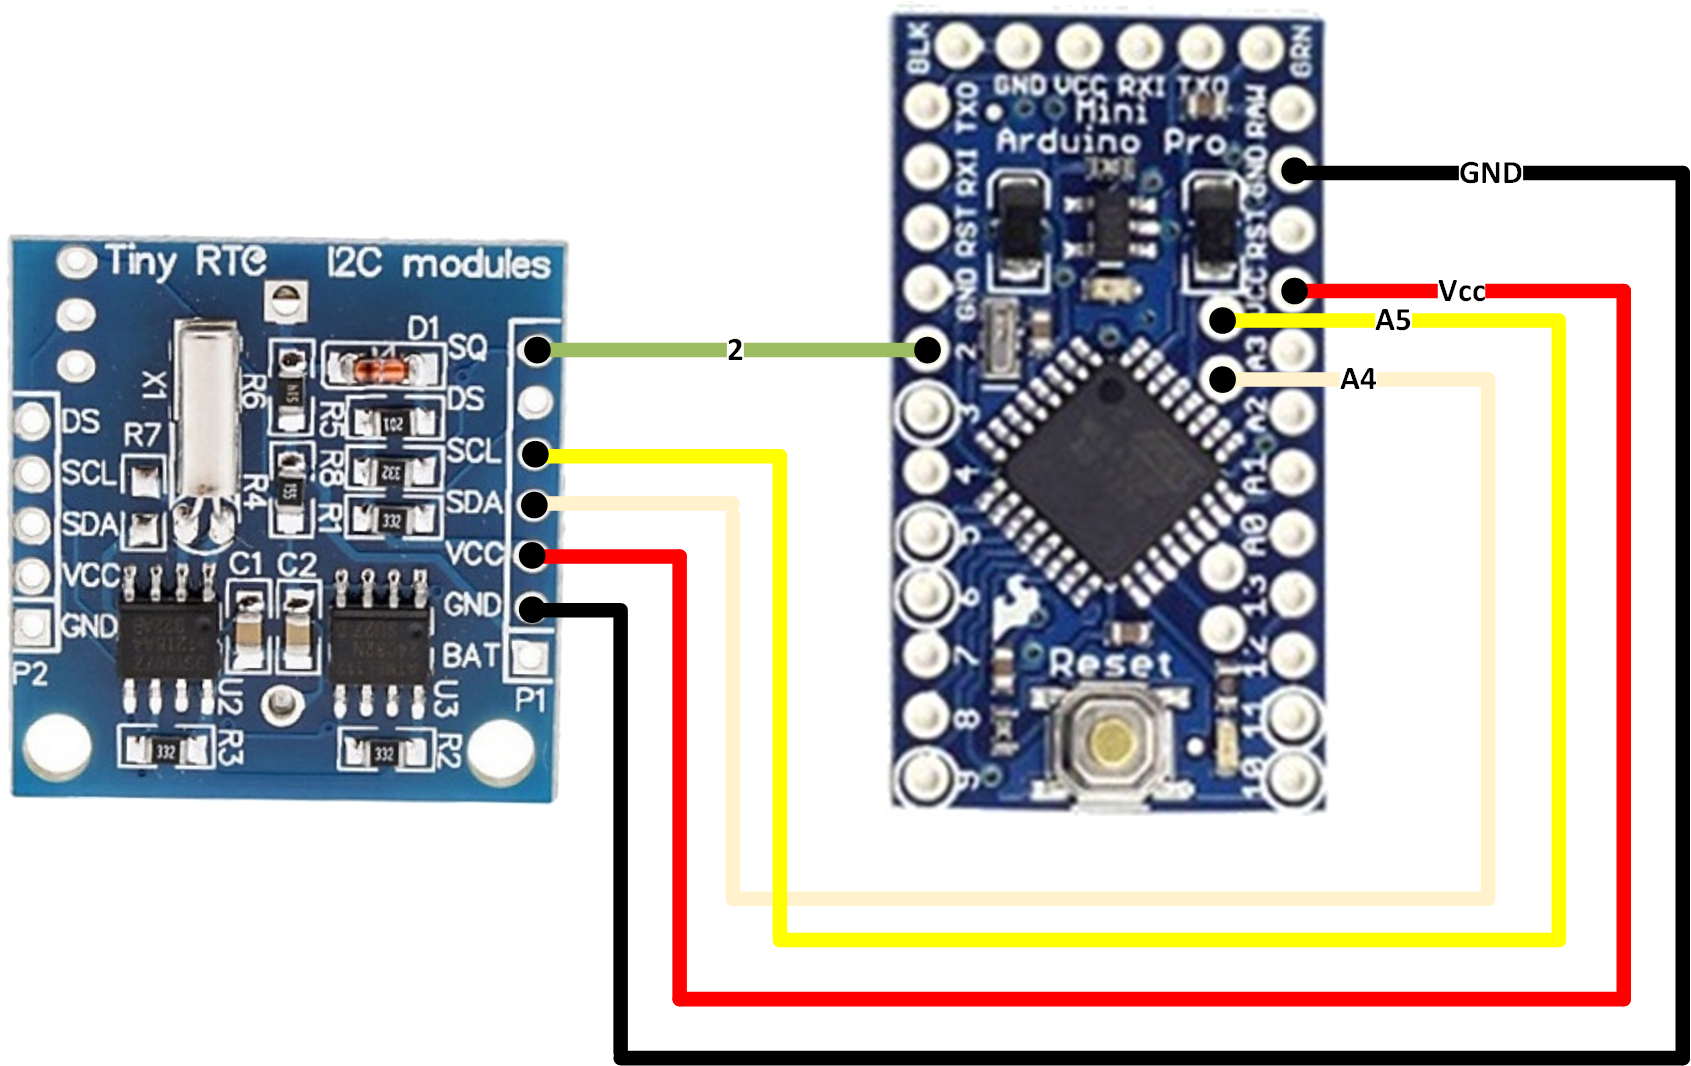
\includegraphics[width=0.85\textwidth]{Figuras/Fig21.png}
\label{fig:fig15}
\end{figure}
%--------------------------------------------------------------------------------

Primeiro executar o exemplo ``SetTime'' que vem nos Exemplos da biblioteca. A seguir, executando o ``ReadTest'' obtem-se a leitura, em intervalos de 1 segundo, do RTC pelo porto série.

%--------------------------------------------------------------------------------
\begin{figure}[htb!]
\centering
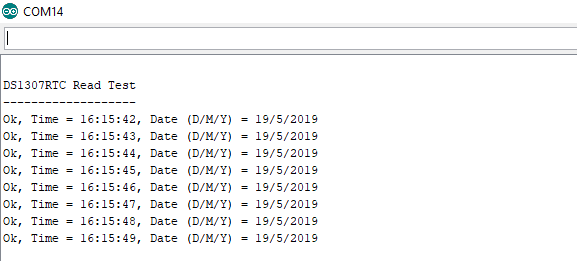
\includegraphics[width=0.65\textwidth]{Figuras/Fig22.png}
\label{fig:fig15}
\end{figure}
%--------------------------------------------------------------------------------

\subsubsection{Update}
A biblioteca referida anteriormente não permite programar a frequência de oscilação da saída SQW do mófulo TinyRTC. Por isso foi isntalada a biblioteca localizada \href{https://github.com/adafruit/RTClib/tree/e03a97139e285eeb4a5a3c052ab421f53a88031c}{aqui}. Tem um exemplo chamado DS1307SqwPin que faz o que é pedido. 

Na Listagem \ref{list4} está um exemplo em que o LED verde da plataforma muda de estado a cada transição descendente do sinal proveniente de SQW.

\lstinputlisting[float, language=Arduino,label=list4,caption=Configura SQW como onda quadrada.]{Codigo/RTCint/RTCint.ino}

Na Listagem \ref{list5}, a data e hora é apresentada na porta série a cada interrupção de 1 segundo.

\lstinputlisting[float, language=Arduino,label=list5,caption=Apresenta data e hora a cada segundo usando interrupção.]{Codigo/ShowTimeWithInterrupt/ShowTimeWithInterrupt.ino}

Esta função tem o problema de não fazer o padding com zeros à esquerda dos números da hora na caso de estes serem inferiores à unidade. De forma a contornar este problema apresentase a Listagem \ref{list6}

\lstinputlisting[float, language=Arduino,label=list6,caption=Apresenta data e hora a cada segundo usando interrupção.]{Codigo/ShowTimeWithInterruptV4/ShowTimeWithInterruptV4.ino}

A versão V4 utiliza 7.216 bytes. A versão anterior ocupa 7.740 bytes e não faz a mesma coisa. Para o conseguir fazer tinha que criar conjuntos de if...then.... o que iria ainda ocupar mais espaço. Por exemplo a Listagem \ref{list7} executa o mesmo que a Listagem \ref{list6} mas ocupa 7.974 bytes.

\lstinputlisting[float, language=Arduino,label=list7,caption=Apresenta data e hora a cada segundo usando interrupção.]{Codigo/ShowTimeWithInterruptV3/ShowTimeWithInterruptV3.ino}

O próximo passo é analisar o comportamento do sistema de armazenamento em cartão SD.

\subsection{SD Card}

%--------------------------------------------------------------------------------
\begin{figure}[htb!]
\centering
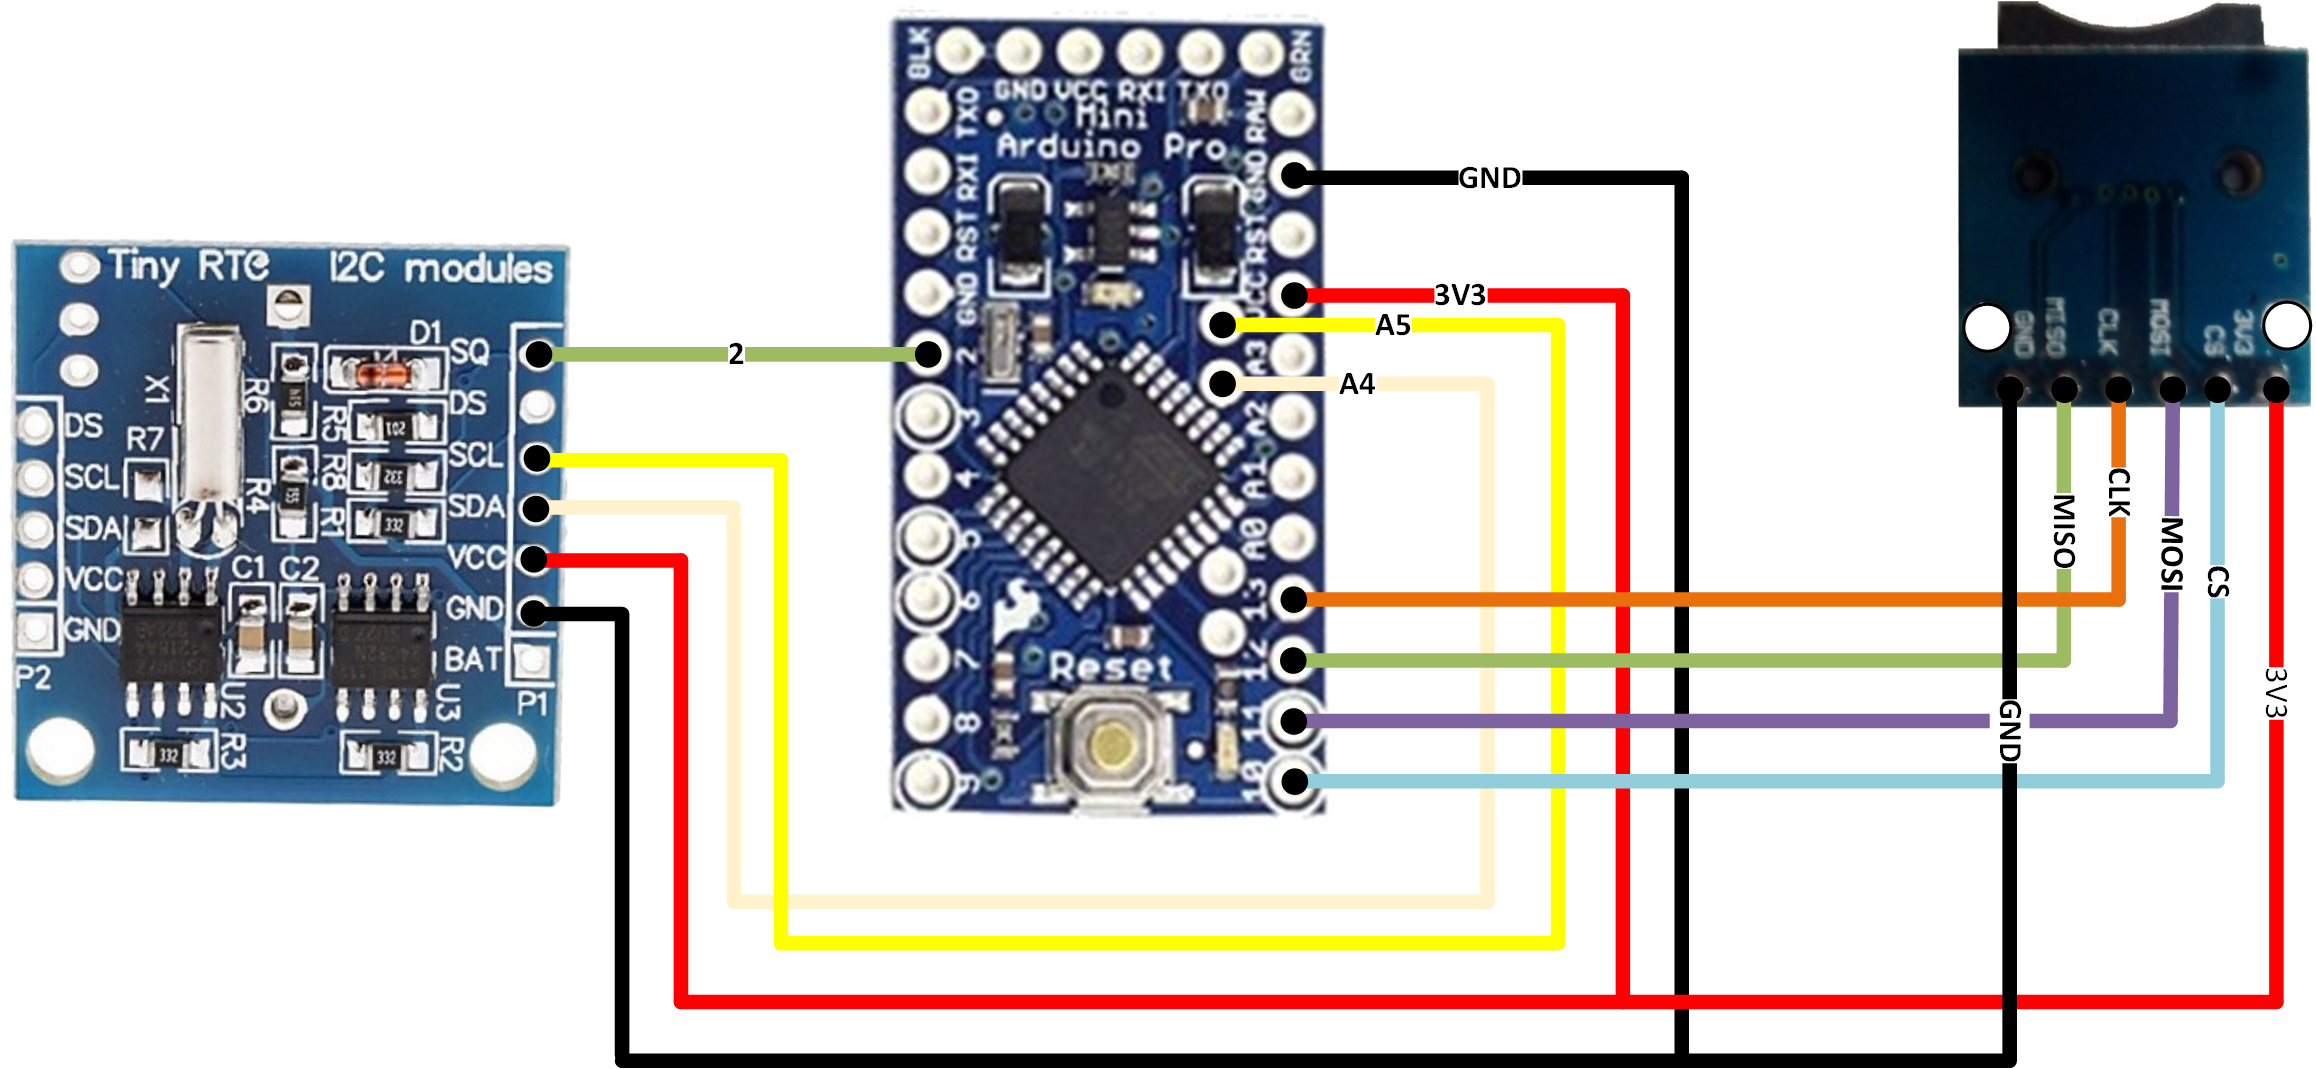
\includegraphics[width=0.8\textwidth]{Figuras/Fig26.png}
\caption{Ligação do SD card}
\label{fig:fig15}
\end{figure}
%--------------------------------------------------------------------------------

%--------------------------------------------------------------------------------
\begin{figure}[htb!]
\centering
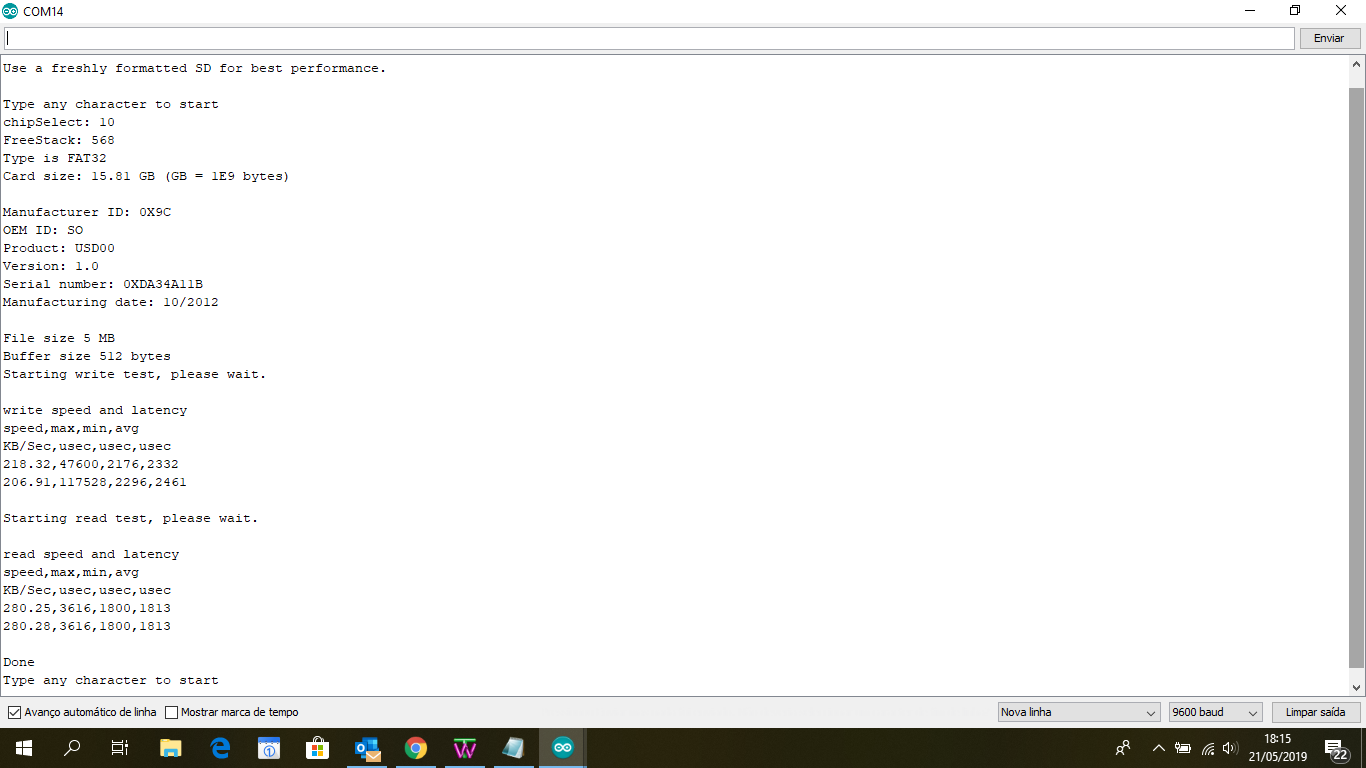
\includegraphics[width=0.8\textwidth]{Figuras/Fig27.png}
\caption{Benchmark do SD card}
\label{fig:fig15}
\end{figure}
%--------------------------------------------------------------------------------

Latencia de escrita (max) = 3~ms

\subsection{Arduino Pro Mini}

Tensão de alimentação em RAW entre 3.3V e 16V aconselhando-se no entanto o uso de tensões entre 4V a 12V. Máxima corrente fornecida pelo regulador : 150~mA. O ATMEGA328 pode fornecer uma corrente máxima, por pino, igual a 40~mA mas o chip, no seu total, não pode fornecer mais de 200~mA. 32kB de memória flash, 1kB de memória E$^2$PROM e 2kB de SRAM.
%--------------------------------------------------------------------------------
\begin{figure}[htb!]
\centering
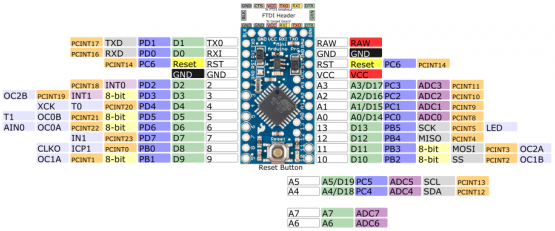
\includegraphics[width=0.8\textwidth]{Figuras/Fig25.png}
\caption{Fonte de alimentação}
\label{fig:fig15}
\end{figure}
%--------------------------------------------------------------------------------


%--------------------------------------------------------------------------------
\begin{figure}[htb!]
\centering
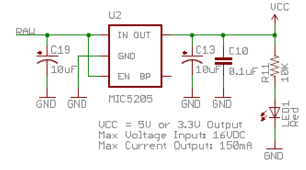
\includegraphics[width=0.4\textwidth]{Figuras/Fig23.png}
\caption{Fonte de alimentação}
\label{fig:fig15}
\end{figure}
%--------------------------------------------------------------------------------
O LED vermelho será removido no final da placa para extender a autonomia.

%--------------------------------------------------------------------------------
\begin{figure}[htb!]
\centering
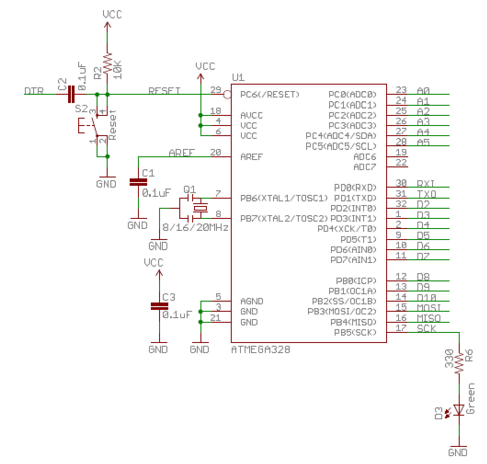
\includegraphics[width=0.6\textwidth]{Figuras/Fig24.png}
\caption{Microcontrolador}
\label{fig:fig15}
\end{figure}
%--------------------------------------------------------------------------------

O LED verde será removido dado que a entrada de SCK será utilizada pelo cartão SD.

\subsection{Qualidade do Conversor DC/DC}

Ripple negligenciável para correntes de 50~mA e 100~mA. 

%+Bibliography
\begin{thebibliography}{99}
\bibitem{Label1} ...
\bibitem{Label2} ...
\end{thebibliography}
%-Bibliography

\end{document}
